\subsection{Branching} % (fold)
\label{sub:branching}

There are two main ways of controlling the sequence of actions in a program. The first of these is called \textbf{branching}, or \textbf{selection}. Branching allows you to get the computer to take one of a number of paths based on the value of a \emph{condition}.

\begin{figure}[h]
   \centering
   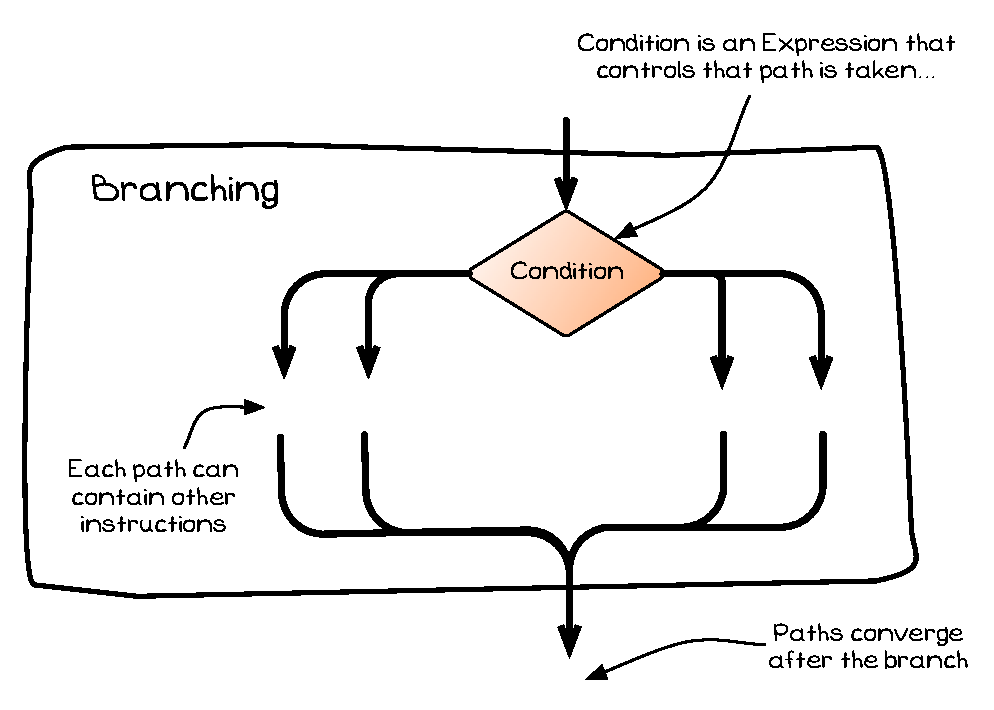
\includegraphics[width=0.8\textwidth]{./topics/control-flow/diagrams/Branching} 
   \caption{Branching commands the computer to take one of a number of possible paths}
   \label{fig:branching}
\end{figure}

\mynote{
\begin{itemize}
  \item Branching is a kind of \textbf{action}. You can command the computer to take of a number of paths.
  \item A branch has a \textbf{condition} that is evaluated, and based on the condition the computer takes one path.
  \item The branch is the act of choosing the path, when its command is performed the computer evaluates the condition and then moves to the instructions in the indicated path.
  \item Languages usually offer two kinds of branching statements:
  \begin{itemize}
    \item \nameref{sub:if_statement} to select between two paths based on a Boolean expression.
    \item \nameref{sub:case_statement}  to select a path based on an ordinal\footnote{Integers and Characters are ordinal values. Ordinal values have a defined sequence, so it is possible to say which value comes next in the sequence. Integers are Ordinal as you can say that the number after 1 is 2. Real numbers are not ordinal as you cannot say which value comes next in the sequence.} value.
  \end{itemize}
  \item The Branch will have one entry point, and one exit point. This feature allows you to combine statements together like building blocks. This idea comes from the principles of \textbf{Structured Programming}, where each component in the code should have a single entry and exit point.
\end{itemize}
}


% subsection branching (end)